\documentclass[10pt,a4paper]{article} %#Establece el tipo de documento y sus especificaciones
%##Lista de paquetes que se podrán usar en el documento
\usepackage[left=2cm,right=2cm,top=2cm,bottom=2cm]{geometry}
\usepackage[dvipsnames]{xcolor}
\usepackage[fleqn]{mathtools}
\usepackage{booktabs}
\usepackage{amsmath}
\usepackage{latexsym}
\usepackage{graphicx}%##Paquete para llamar imagenes
\usepackage{nccmath}
\usepackage{multicol}
\usepackage{listings}
\usepackage{tasks}
\usepackage{color}
\usepackage{float}
\usepackage{lipsum}
\usepackage[spanish]{babel}
\UseRawInputEncoding

\definecolor{colorIPN}{rgb}{0.5, 0.0,0.13}
\definecolor{colorESCOM}{rgb}{0.0, 0.5,1.0}
\graphicspath{ {imagenes/} }

\begin{document} %##Indica donde inicia el documento
	%#########################################################
	\begin{titlepage}
		\centering
		{ \huge \bfseries \color{colorIPN}{Instituto Politécnico Nacional} \par}
		{ \Large \bfseries  \color{colorESCOM}{Escuela Superior de C{\' o}mputo} \par }
		\vspace{1cm}%##Inserta una separación de tamaño exacto entre líneas
		{\huge\Large \color{colorIPN}{Web App Development}.\par}
		\vspace{1.5cm}
		{\huge\Large  \color{colorESCOM}{Ejercicio 3 : Registro en Heroku}\par}
		\vspace{2cm}
		{\Large\itshape \color{colorIPN}{Profesor: M. en C. Jos{\' e} Asunci{\' o}n Enr{\' i}quez Z{\' a}rate}\par} \hfill \break
		\vspace{2cm}
		{\Large\itshape \color{colorIPN}{Alumno: Mauro Sampayo Hern{\' a}ndez}\par} \hfill \break
		{\Large\itshape \color{colorIPN}{mauro\_luigi@hotmail.com}\par} \hfill \break
		{\Large\itshape \color{colorIPN}{3CM18} \par}
		\vfill
		{\large \color{colorIPN}{\today}\par} 
		\vfill
	\end{titlepage}
	
	\renewcommand\lstlistingname{Quelltext} 
	
	\settasks{
		counter-format=(tsk[r]),
		label-width=4ex
	}
	\tableofcontents 
	\pagebreak
	
	\pagenumbering {arabic} %##Coloca el contador de páginas a 1 y comienza a numerar de acuerdo con el estilo especificado. En este caso dicho estilo de numeracion es el arabigo
	
	\pagebreak
	
	%################################################
	\section{\color{colorIPN}{Introducci{\' o}n}}%##Crea secciones númeradas, en este caso esta es la seccion 1
	{\large Heroku es una plataforma basada en la nube como servicio (PaaS) dise{\~n}ada para que los desarrolladores y equipos creen, env{\'i}en, supervisen y escalen aplicaciones modernas. Esta plataforma brinda a los desarrolladores mayor tiempo para centrarse en el producto principal sin tener que preocuparse de mantener la infraestructura de la aplicaci{\'o}n.  
		
		
		\vspace{0.5cm}
		Heroku adem{\'a}s ofrece herramientas, servicios y flujos de trabajo integrados para ayudar a las organizaciones de todos los tama{\~n}os a maximizar la productividad individual y del equipo para poder entregar aplicaciones en el mercado m{\'a}s r{\'a}pidamente.
		
		\vspace{0.5cm}
		En este reporte se mostrar{\'a} el proceso a seguir, para realizar el registro en esta plataforma y poder usar los beneficios que nos brinda.}
	
	%\subsection{ \color{colorESCOM}{Sub Sección 1}} %##Crea subsecciones numeradas
	%\lipsum[2-3] %##Añade tecto lorem ipsum
	
	\pagebreak
	
	%################################################
	\section{\color{colorIPN}{Conceptos}}
	
	\subsection{ \color{colorESCOM}{Inform{\'a}tica en la nube}}
	{\large La inform{\'a}tica en la nube es el suministro de servicios inform{\'a}ticos (incluidos servidores, almacenamiento, bases de datos, redes, software, an{\'a}lisis e inteligencia) a trav{\'e}s de Internet (la nube), cuyo objetivo es ofrecer una innovaci{\'o}n m{\'a}s r{\'a}pida, recursos flexibles y econom{\'i}as de escala.
		
		
		\vspace{0.5cm}
		La mayor{\'i}a de los servicios de inform{\'a}tica en la nube se engloban en cuatro categor{\'i}as generales: infraestructura como servicio (IaaS), plataforma como servicio (PaaS), sin servidor y software como servicio (SaaS).
		
		
		\vspace{0.5cm}
		Existen 3 tipos de nubes inform{\'a}ticas:}
	
	\subsubsection{\color{colorESCOM}{Nubes p{\'u}blicas:}}
	{\large Los recursos en la nube (como los servidores y el almacenamiento) son propiedad de un proveedor de servicios en la nube que los administra y los ofrece a trav{\'e}s de Internet. Con una nube p{\'u}blica, todo el hardware, el software y los dem{\'a}s componentes de la infraestructura subyacente son propiedad del proveedor de nube, que tambi{\'e}n los administra. }
	
	\subsubsection{\color{colorESCOM}{Nubes privadas:}}
	{\large Una nube privada est{\'a} compuesta por recursos inform{\'a}ticos en la nube que utiliza exclusivamente una empresa u organizaci{\'o}n. La nube privada puede ubicarse f{\'i}sicamente en el centro de datos local de su organizaci{\'o}n u hospedarla un proveedor de servicios externo. Sin embargo, en una nube privada, los servicios y la infraestructura siempre se mantienen en una red privada, y el hardware y software se dedican {\'u}nicamente a su organizaci{\'o}n. }
	
	\subsubsection{\color{colorESCOM}{Nubes hibridas:}}
	{\large Es la mezcla de servicios de nube p{\'u}blica y servicios de nube privada. 
		
		
		\vspace{0.5cm}}
	
	
	\subsection{ \color{colorESCOM}{Plataforma como Servicio (PAAS):}}
	{\large Es un entorno de desarrollo e implementaci{\'o}n completo en la nube, con recursos que permiten entregar todo, desde aplicaciones sencillas basadas en la nube hasta aplicaciones empresariales sofisticadas habilitadas para la nube.
		
		
		\vspace{0.5cm}
		PaaS incluye infraestructura (servidores, almacenamiento y redes), middleware, herramientas de desarrollo, servicios de inteligencia empresarial, sistemas de administraci{\'o}n de bases de datos, etc. PaaS est{\'a} dise{\~n}ado para sustentar el ciclo de vida completo de las aplicaciones web: compilaci{\'o}n, pruebas, implementaci{\'o}n, administraci{\'o}n y actualizaci{\'o}n.}
	
	\pagebreak
	
	%################################################
	\section{\color{colorIPN}{Desarrollo}}
	{\large Para el desarrollo de este ejercicio se mostrar{\' a} el proceso a seguir para poder registrarse en la Plataforma Heroku:}
	
	\begin{enumerate}
		{\large
			\item Como primer paso se debe de ingresar a la liga \underline{https://signup.heroku.com/} la cu{\'a}l nos redirecciona a la p{\'a}gina de Heroku donde se podr{\'a} realizar el registro a el servicio que ofrece Heroku.
			\begin{figure}[H]
				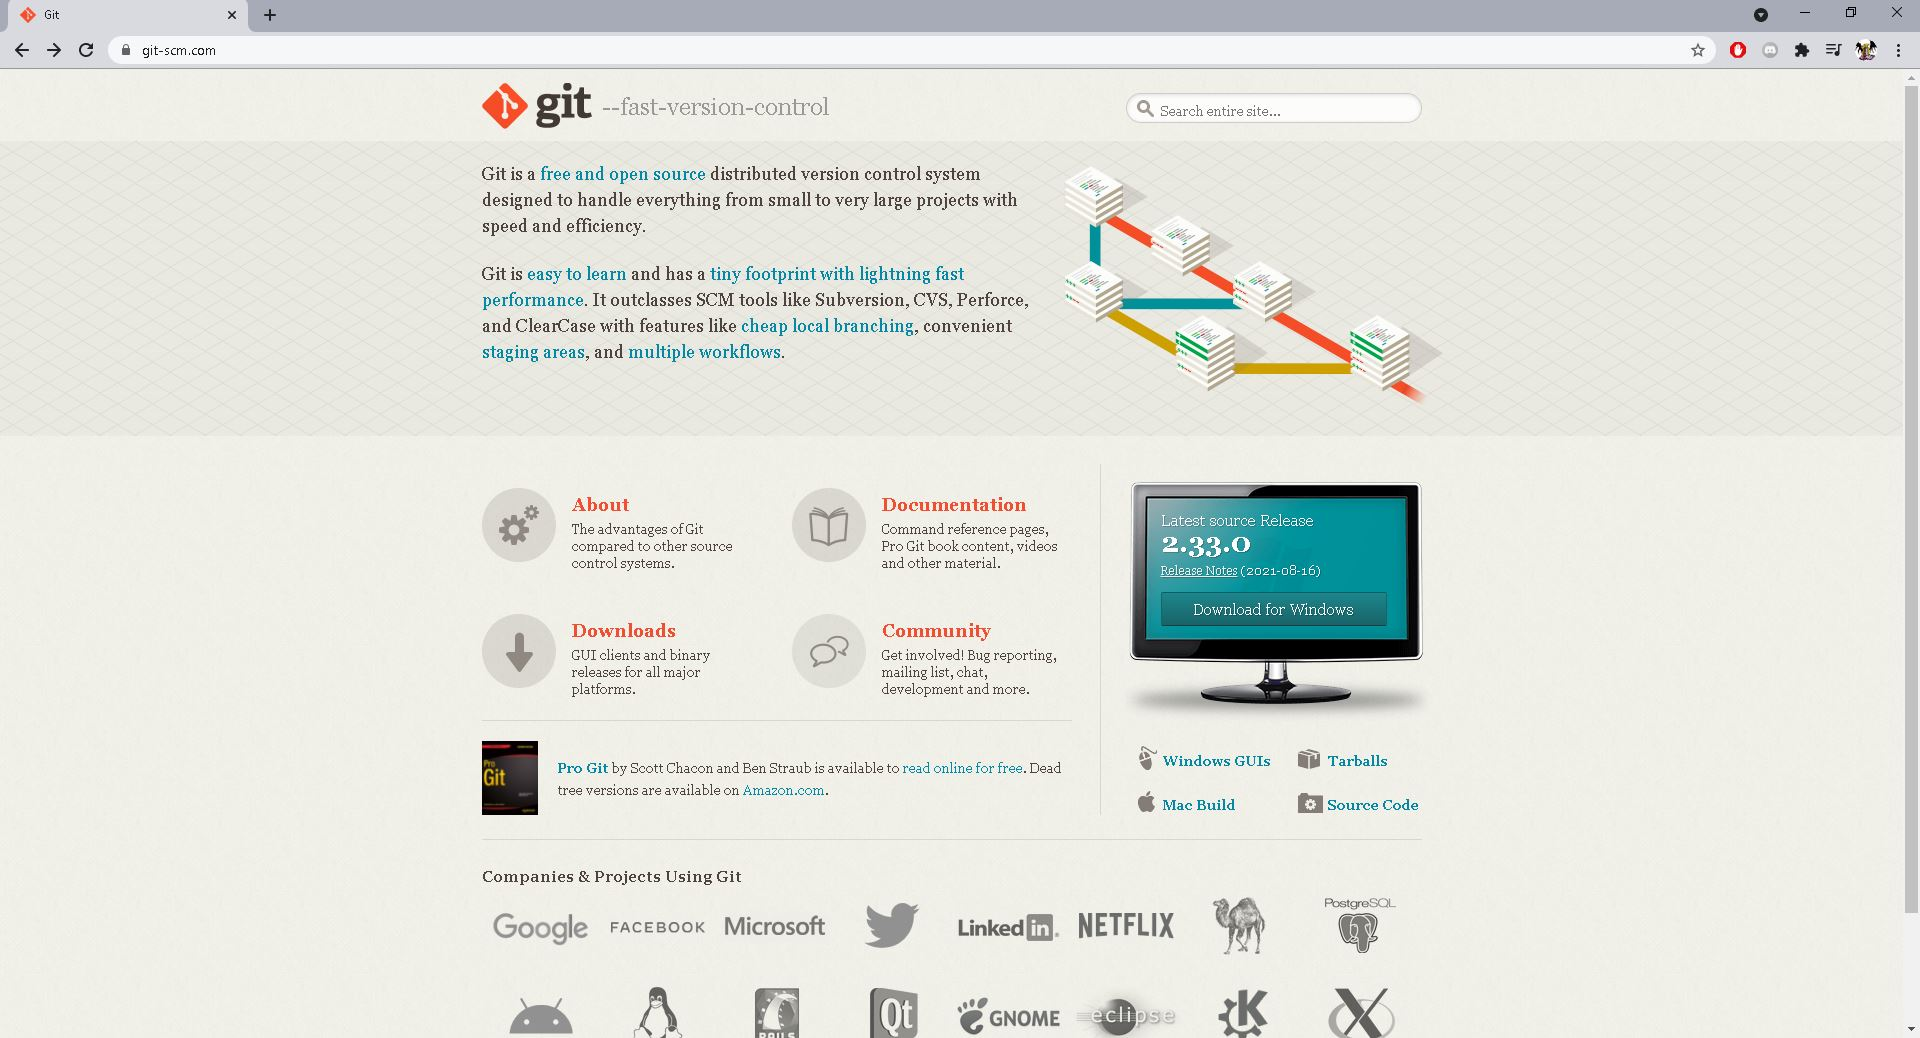
\includegraphics[width=0.9\textwidth]{1.jpg}
				\centering
				\label{img:paso1}
			\end{figure}
			\item Para poder realizar el registro deberemos rellenar el formulario que se nos solicita en la p{\'a}gina. Los datos que se nos solicitan son el Nombre, apellidos, correo electr{\'o}nico, nombre de la compa{\~n}{\'i}a para la que se trabaja (solo en caso de que el usuario este trabajando para una, de lo contrario el campo se puede dejar sin rellenar), rol, pa{\'i}s y el lenguaje de programaci{\'o}n que el usuario utilizar{\'a} para hacer uso de los servicios proporcionados por Heroku (para el caso de esta materia dicho lenguaje es Java. A continuaci{\'o}n, se muestra un ejemplo de como debe ser llenado este formulario.
			\begin{figure}[H]
				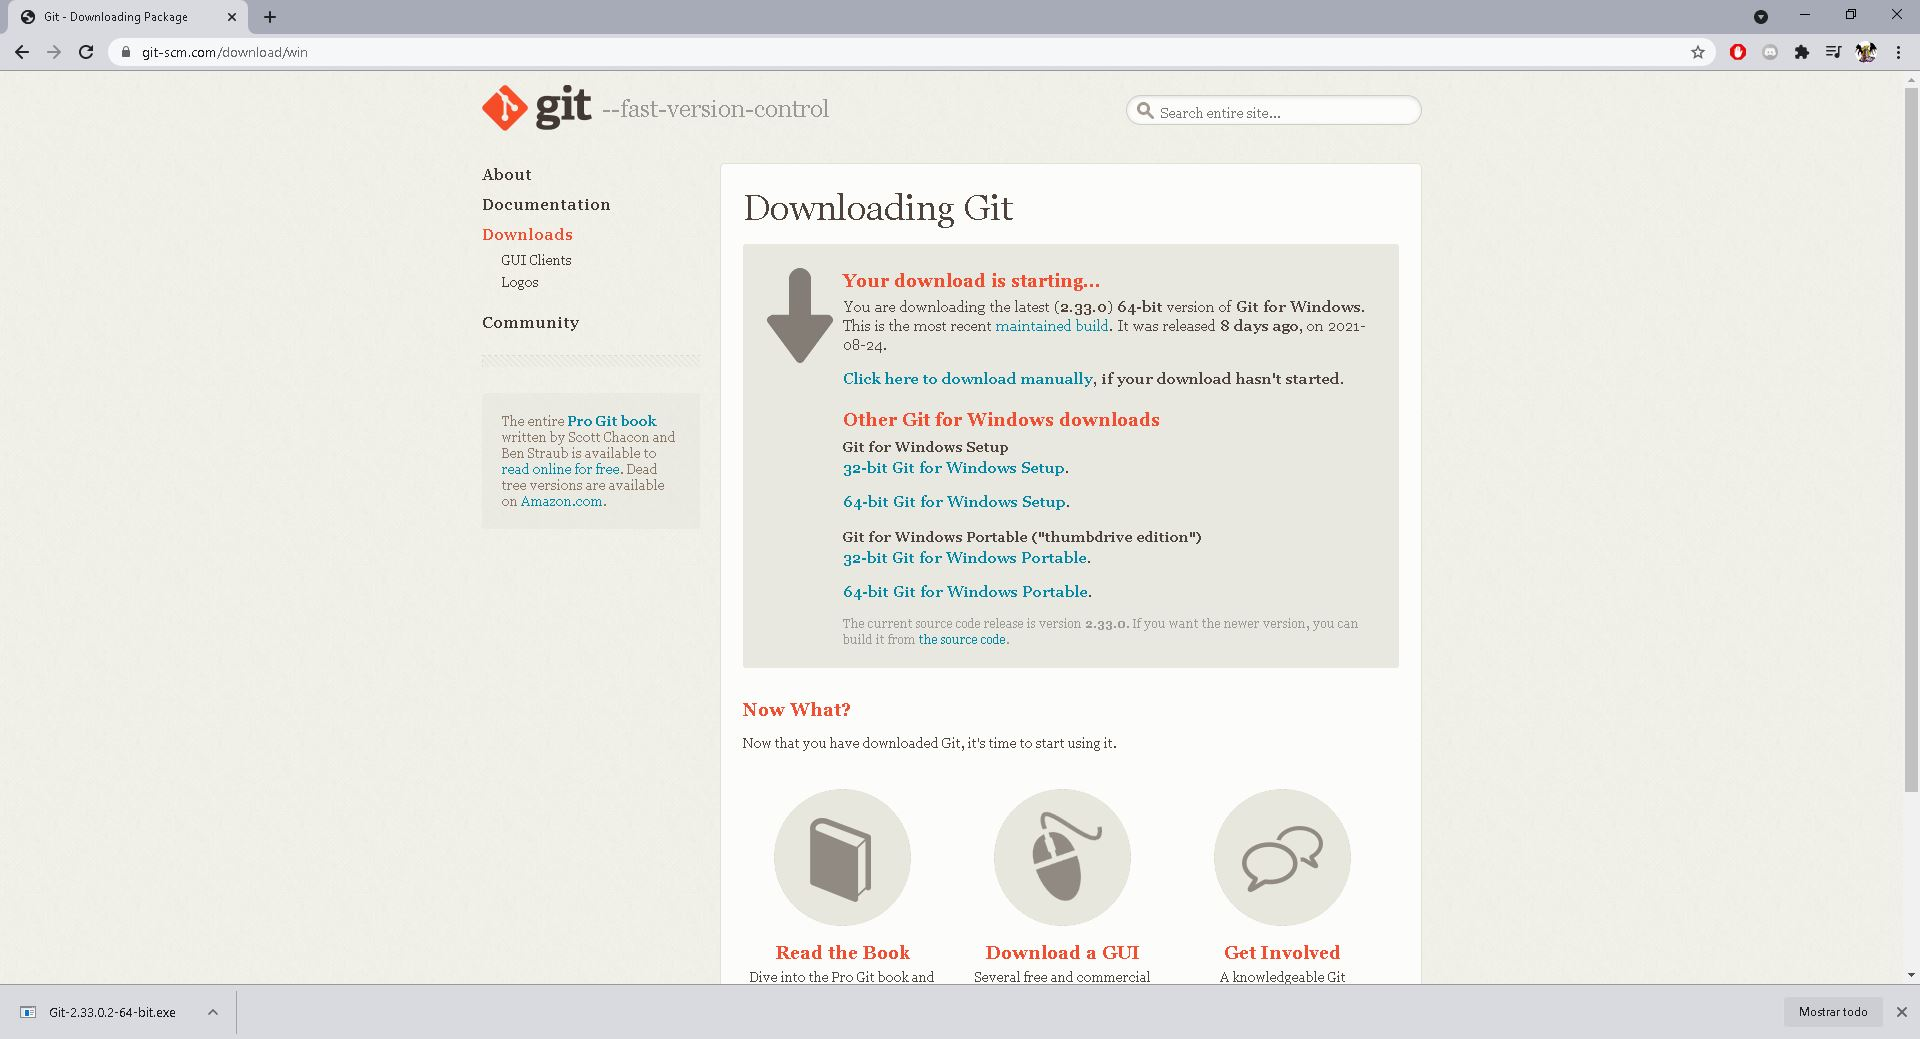
\includegraphics[width=0.9\textwidth]{2.jpg}
				\centering
				\label{img:paso2}
			\end{figure}
			
			\pagebreak
			Una vez se haya finalizado de rellenar los campos del formulario, debemos realizar el captcha para verificar que somos humanos, y despu{\'e}s seleccionar la opci{\'o}n ``Create free account''.
			
			\item Posteriormente la p{\'a}gina de Heroku nos notificar{\'a} que ha sido enviado un correo electr{\'o}nico a la direcci{\'o}n de correo que ingresamos en el formulario para verificar y activar nuestra cuenta. Se deber{\'a} acceder a dicho correo y dar click al enlace que se nos indica en el mismo, para realizar la activaci{\'o}n de la cuanta de Heroku. Cabe resaltar que tendremos un m{\'a}ximo de 30 d{\'i}as para realizar este proceso.
			\begin{figure}[H]
				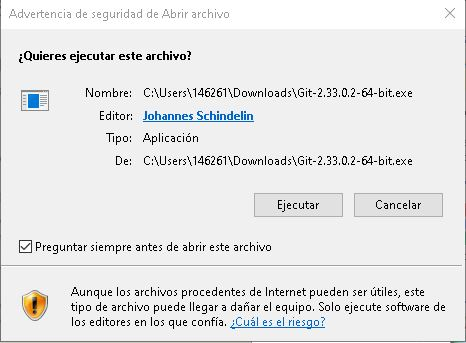
\includegraphics[width=0.9\textwidth]{3.jpg}
				\centering
				\label{img:paso3}
				
				
				\vspace{0.5cm}
				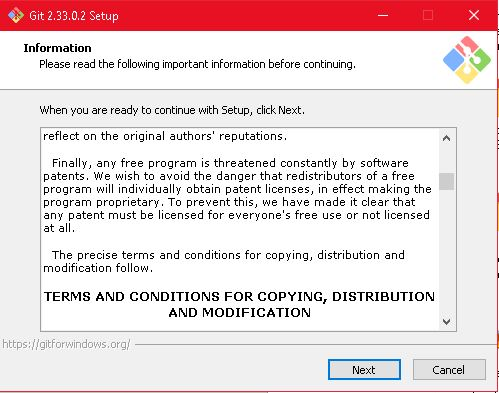
\includegraphics[width=0.8\textwidth]{4.jpg}
				\centering
				\label{img:paso4}
			\end{figure}
			
			\pagebreak
			\item Una vez realizada la activaci{\'o}n de nuestra cuenta, se nos solicitar{\'a} que ingresemos una contrase{\~n}a para la misma. Una vez ingresada la contrase{\~n}a se debe seleccionar la opci{\'o}n de ``Set Password and Log In''.
			\begin{figure}[H]
				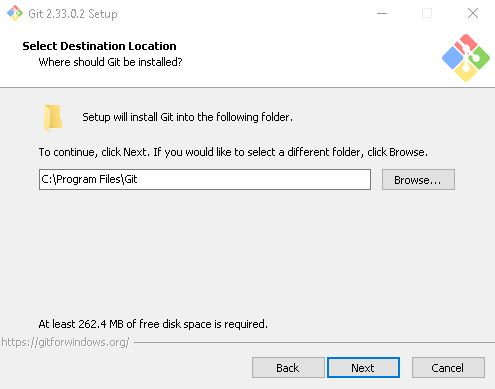
\includegraphics[width=0.9\textwidth]{5.jpg}
				\centering
				\label{img:paso5}
			\end{figure}
			\item Heroku nos dar{\'a} la bienvenida a la plataforma y nos indicar{\'a} que nuestra cuenta ha sido creada exitosamente.
			\begin{figure}[H]
				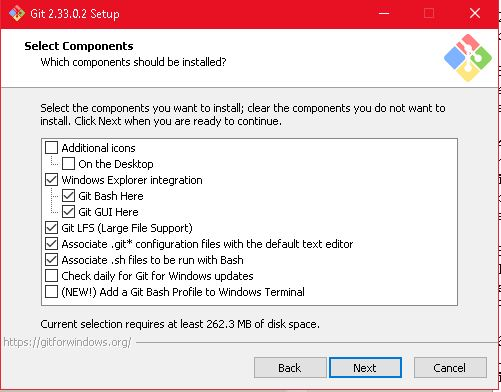
\includegraphics[width=0.9\textwidth]{6.jpg}
				\centering
				\label{img:paso6}
			\end{figure}
			
			\pagebreak
			\item Opcionalmente Heroku nos da la posibilidad de a{\~n}adir una capa extra de seguridad para que nuestra cuenta tenga una mayor protecci{\'o}n. Para este caso no se mostrar{\'a} este proceso.
			\begin{figure}[H]
				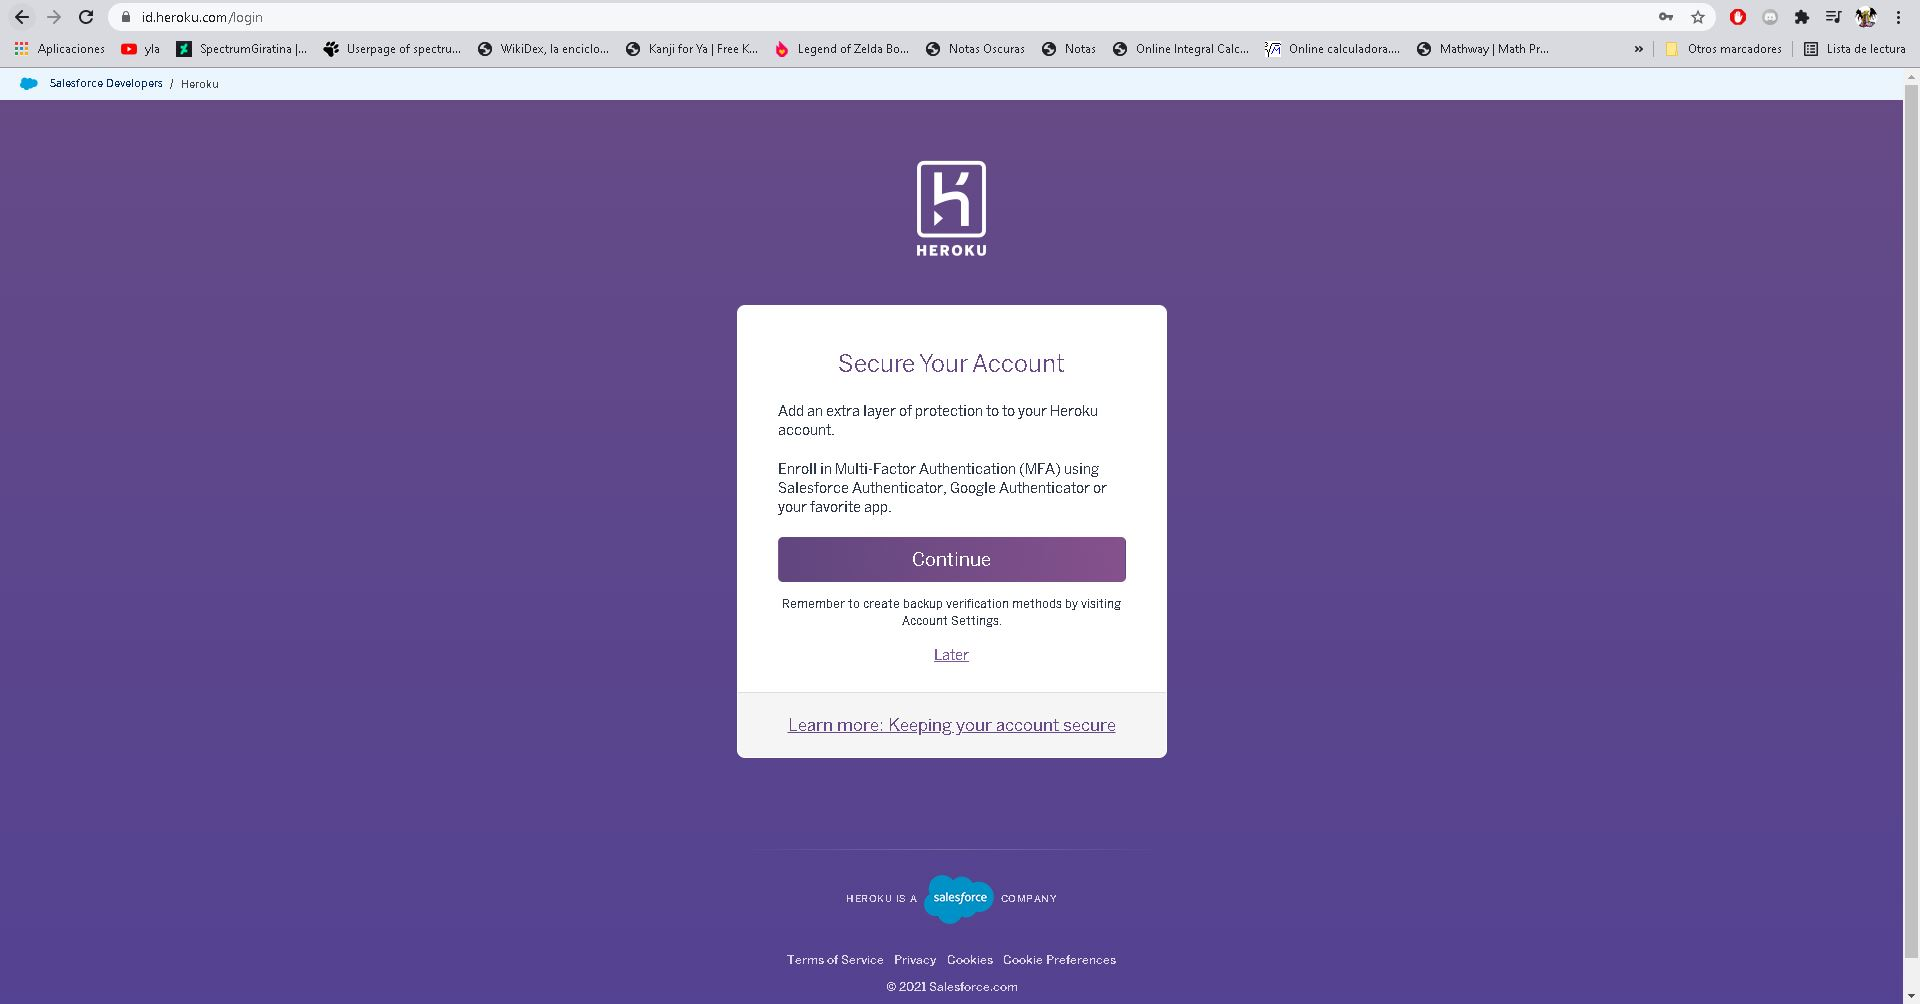
\includegraphics[width=0.9\textwidth]{7.jpg}
				\centering
				\label{img:paso7}
			\end{figure}
			\item Como paso final, se deber{\'a}n aceptar los T{\'e}rminos y Condiciones de Heroku.
			\begin{figure}[H]
				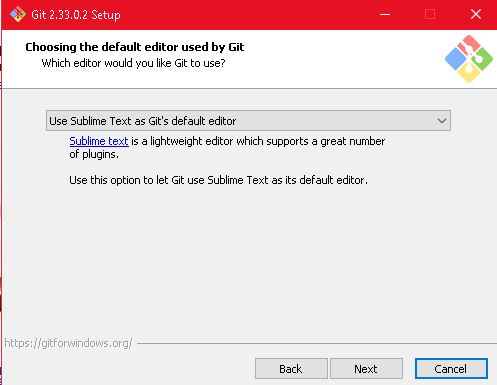
\includegraphics[width=0.9\textwidth]{8.jpg}
				\centering
				\label{img:paso8}
			\end{figure}
		}
	\end{enumerate}
	
	\pagebreak
	
	%################################################
	\section{\color{colorIPN}{Resultados}}
	{\large Tras haber finalizado la verificaci{\'o}n y activaci{\'o}n de la cuenta, y haber aceptado los T{\'e}rminos y Condiciones del producto, tendremos acceso finalmente a la plataforma web de Heroku, la cu{\'a}l nos provee con diversas opciones y herramientas para la creaci{\'o}n de aplicaciones, adem{\'a}s de brindarnos con diversas gu{\'i}as para poder realizar el despliegue de las aplicaciones que desarrollemos en la plataforma, desde diversos lenguajes de programaci{\'o}n.}
	
	\begin{figure}[H]
		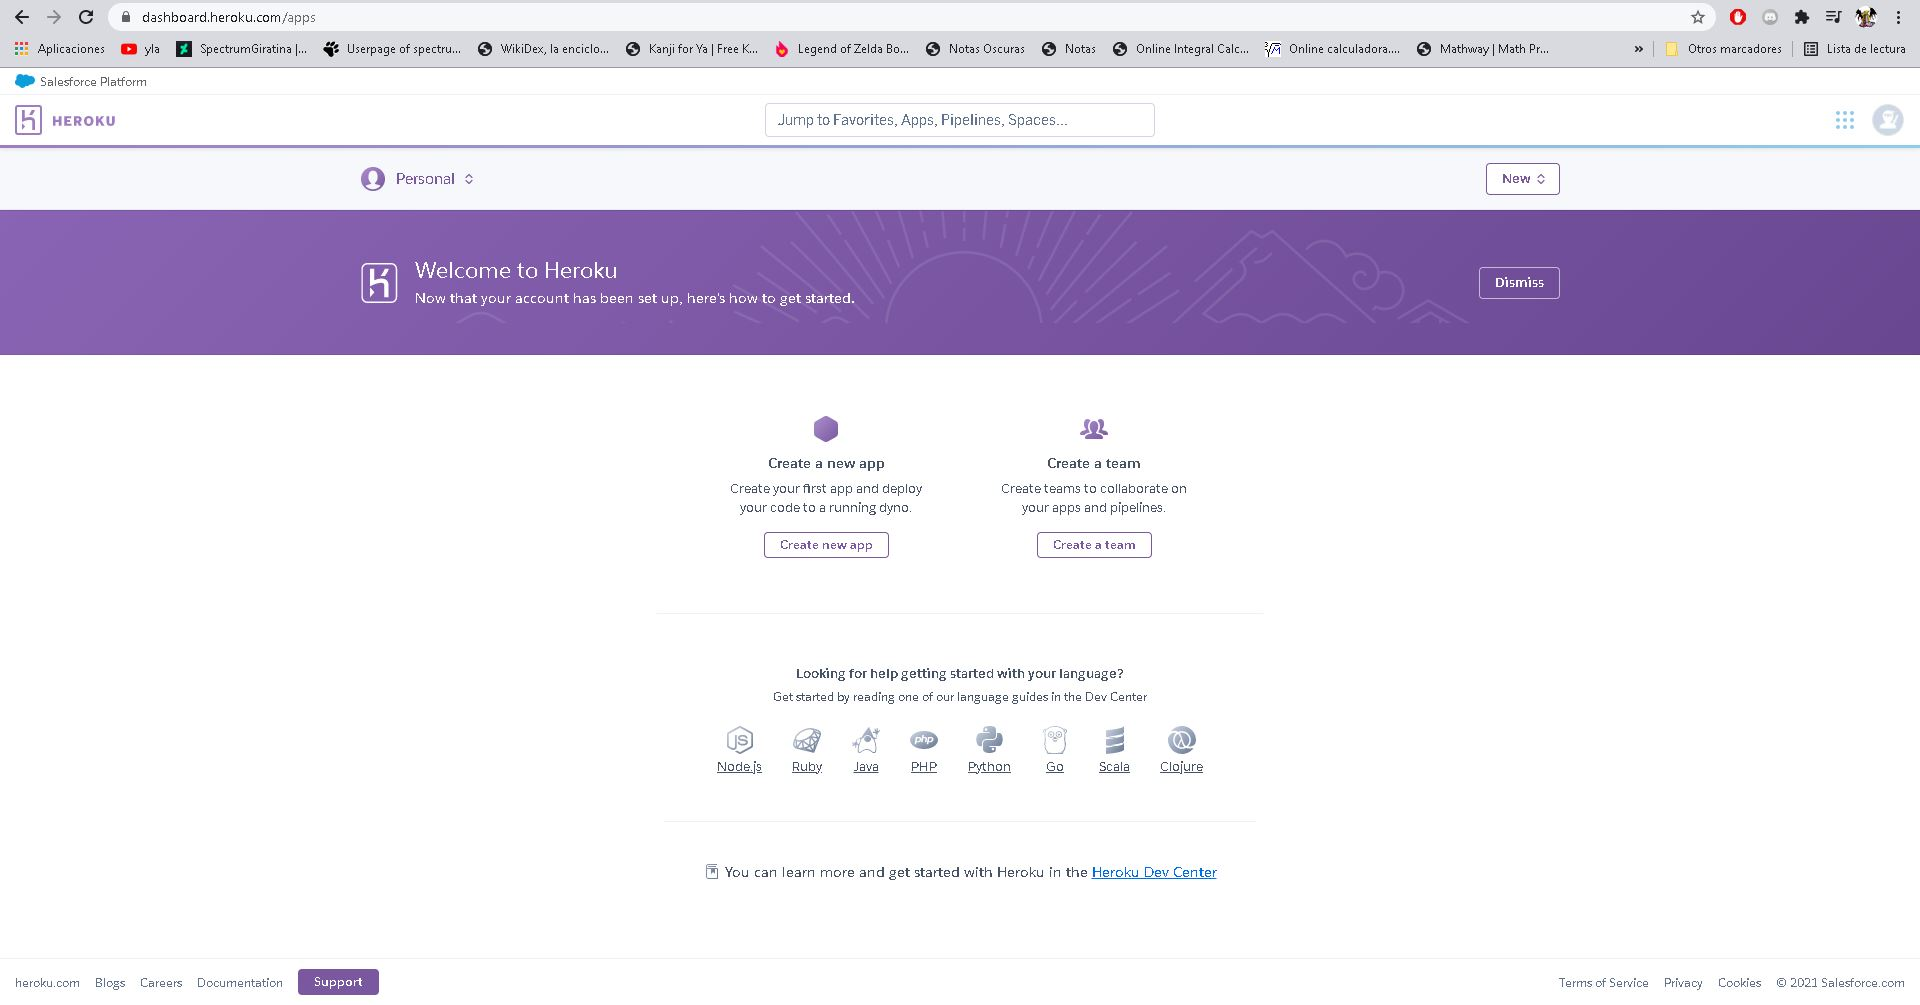
\includegraphics[width=\textwidth]{resultado.jpg}
		\centering
		\label{img:resultado}
	\end{figure}
	
	\pagebreak
	
	
	%################################################
	\section{\color{colorIPN}{Conclusi{\' o}n}}
	{\large Heroku es una plataforma bastante {\'u}til en tanto a el desarrollo de apliciones, pues adem{\'a}s de brindarnos con una interfaz f{\'a}cil de entender y gu{\'i}as para poder desplegar aplicaciones desde distintos lenguajes de programaci{\'o}n; a nivel organizacional permite a los desarrolladores un desarrollo mucho m{\'a}s fluido y r{\'a}pido de aplicaciones, lo cu{\'a}l significa un aumento de la productividad de la misma organizaci{\'o}n y un aumento en la eficiencia de la misma organizaci{\'o}n.}
	
	\color{colorIPN}{
		\begin{flushright}
			\textit{
				Mauro Sampayo Hern{\' a}ndez
			}
		\end{flushright} \hfill \break
	}
	
	\pagebreak
	
	%################################################
	
	\section{\color{colorIPN}{Referencias Bibliográficas}}
	\color{colorESCOM}{
		\begin{thebibliography}{10}
			\bibitem {heroku}
			\newblock {\em Sobre Heroku}
			\newblock \textbf {GetApp.}
			\newblock [accesed 2021 Sep 19]
			\newblock {\em https://www.getapp.com.mx/software/113509/heroku1}
			
			\bibitem {PaaS}
			\newblock {\em ?`Qu{\'e} es PaaS?}
			\newblock \textbf {Microsoft Azure}
			\newblock [accesed 2021 Sep 19]
			\newblock {\em https://azure.microsoft.com/es-mx/overview/what-is-paas/}
			
			\bibitem {nube}
			\newblock {\em ?`Qu{\'e} es la inform{\'a}tica en la nube?}
			\newblock \textbf {Microsoft Azure}
			\newblock [accesed 2021 Sep 19]
			\newblock {\em https://azure.microsoft.com/es-mx/overview/what-is-cloud-computing/\#benefits}
			
			\bibitem {tipoNubes}
			\newblock {\em ?`Qu{\'e} es la nube p{\'u}blica, privada e h{\'i}brida?}
			\newblock \textbf {Microsoft Azure}
			\newblock [accesed 2021 Sep 19]
			\newblock {\em https://azure.microsoft.com/es-es/overview/what-are-private-public-hybrid-clouds/\#overview}
			
			\bibitem {creacionCuenta}
			\newblock {\em Crear Cuenta en Heroku}
			\newblock [accesed 2021 Sep 19]
			\newblock {\em https://www.youtube.com/watch?v=OX1yjl7V4L8\&ab\_channel =SolucionsSistemas}
		\end{thebibliography}
	}
	
\end{document} %##Indica donde termina el documento